\chapter{A Classical Approach to Data Acquisition System Design}
\label{chap:III-1-arch}

  In the early development stages of the DAQ system for the GE1/1 detector, before the first version of the OptoHybrid was designed, a small prototyping setup was developed to readout a 10 cm $ \times $ 10 cm Triple-GEM detector using VFAT2 Hybrids. With time, the setup was improved to use the GLIB and later on the OptoHybrid. Next to the data readout chain, the system also controls the high voltage and gas sources from a web interface. \\

  In this chapter, we describe the evolution of the DAQ system developed to read out a small Triple-GEM prototype. We describe the technologies that have been used and the developments that were performed in order to integrate the components in the system.

  \section{The Experimental Setup}

    The experimental setup consists of a 10 cm $ \times $ 10 cm Triple-GEM detector placed between two scintillators which coincidence is used to produce triggers. The GEM prototype is equipped with a two-dimensional readout board with 2 times 128 strips in each direction. Figure \ref{fig:III-1-gem} is a photograph of the detector showing the four readout connector, the high voltage resistive divider in the bottom left, and the gas supply in the bottom right. \\

    \begin{figure}[h!]
      \centering
      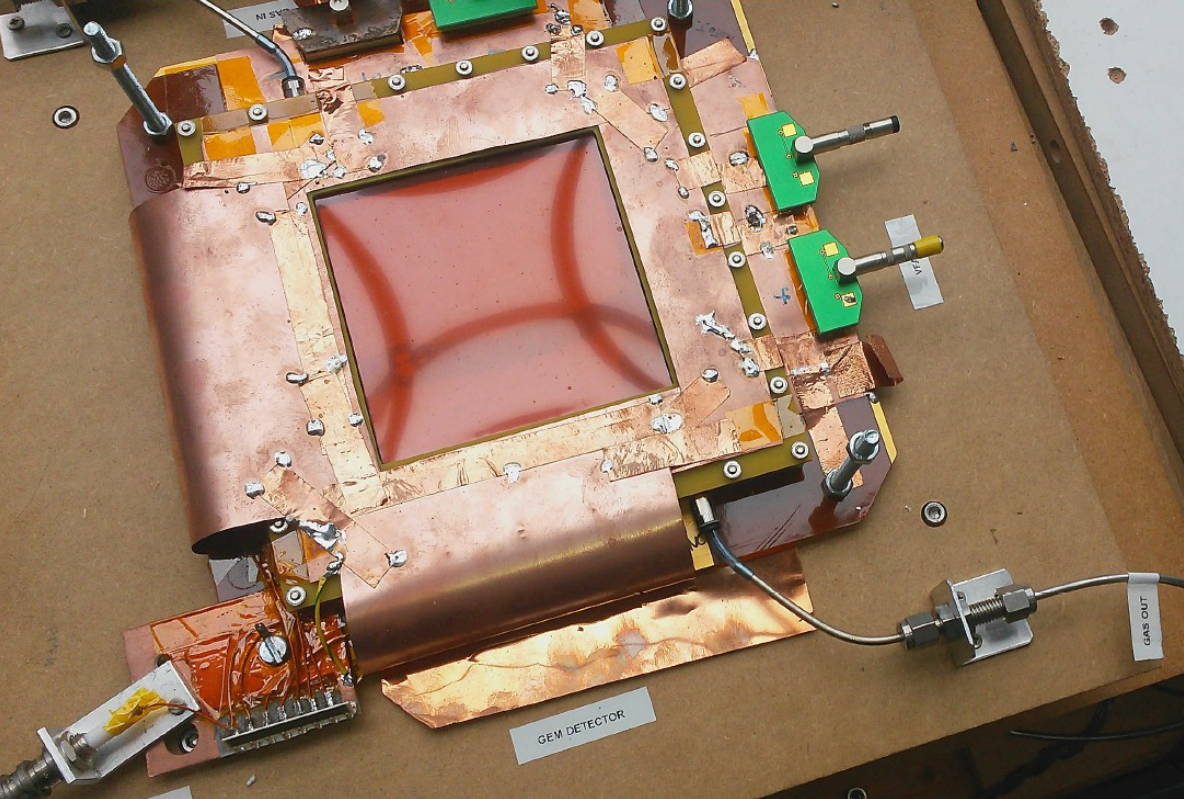
\includegraphics[width=0.8\textwidth]{img/III-1-arch/gem.png}
      \caption{}
      \label{fig:III-1-gem}
    \end{figure}

    The high voltage provided to the GEM and the photomultipliers attached to the scintillators is originating from a CAEN V6533N VME module. VME is a crate standard that defines a high speed communication protocol and an infrastructure for the interconnect of the boards. A CAEN V1718 VME-USB bridge board is used to control the communication of the VME crate from a computer. This modules allows the latter to talk to any board in the crate by initiating requests. The gas flow is regulated by four HORIBA STEC SEC-N112MGRW mass flow controllers: three for the Ar, CO$_2$, and CF$_4$ gas bottles and one to monitor the mixture. These are controlled through a serial link communication by a computer. Figure \ref{fig:III-1-gas-hv} shows photographs of the VME high-voltage module on the left and the mass flow meters on the right.

    \begin{figure}[h!]
      \centering
      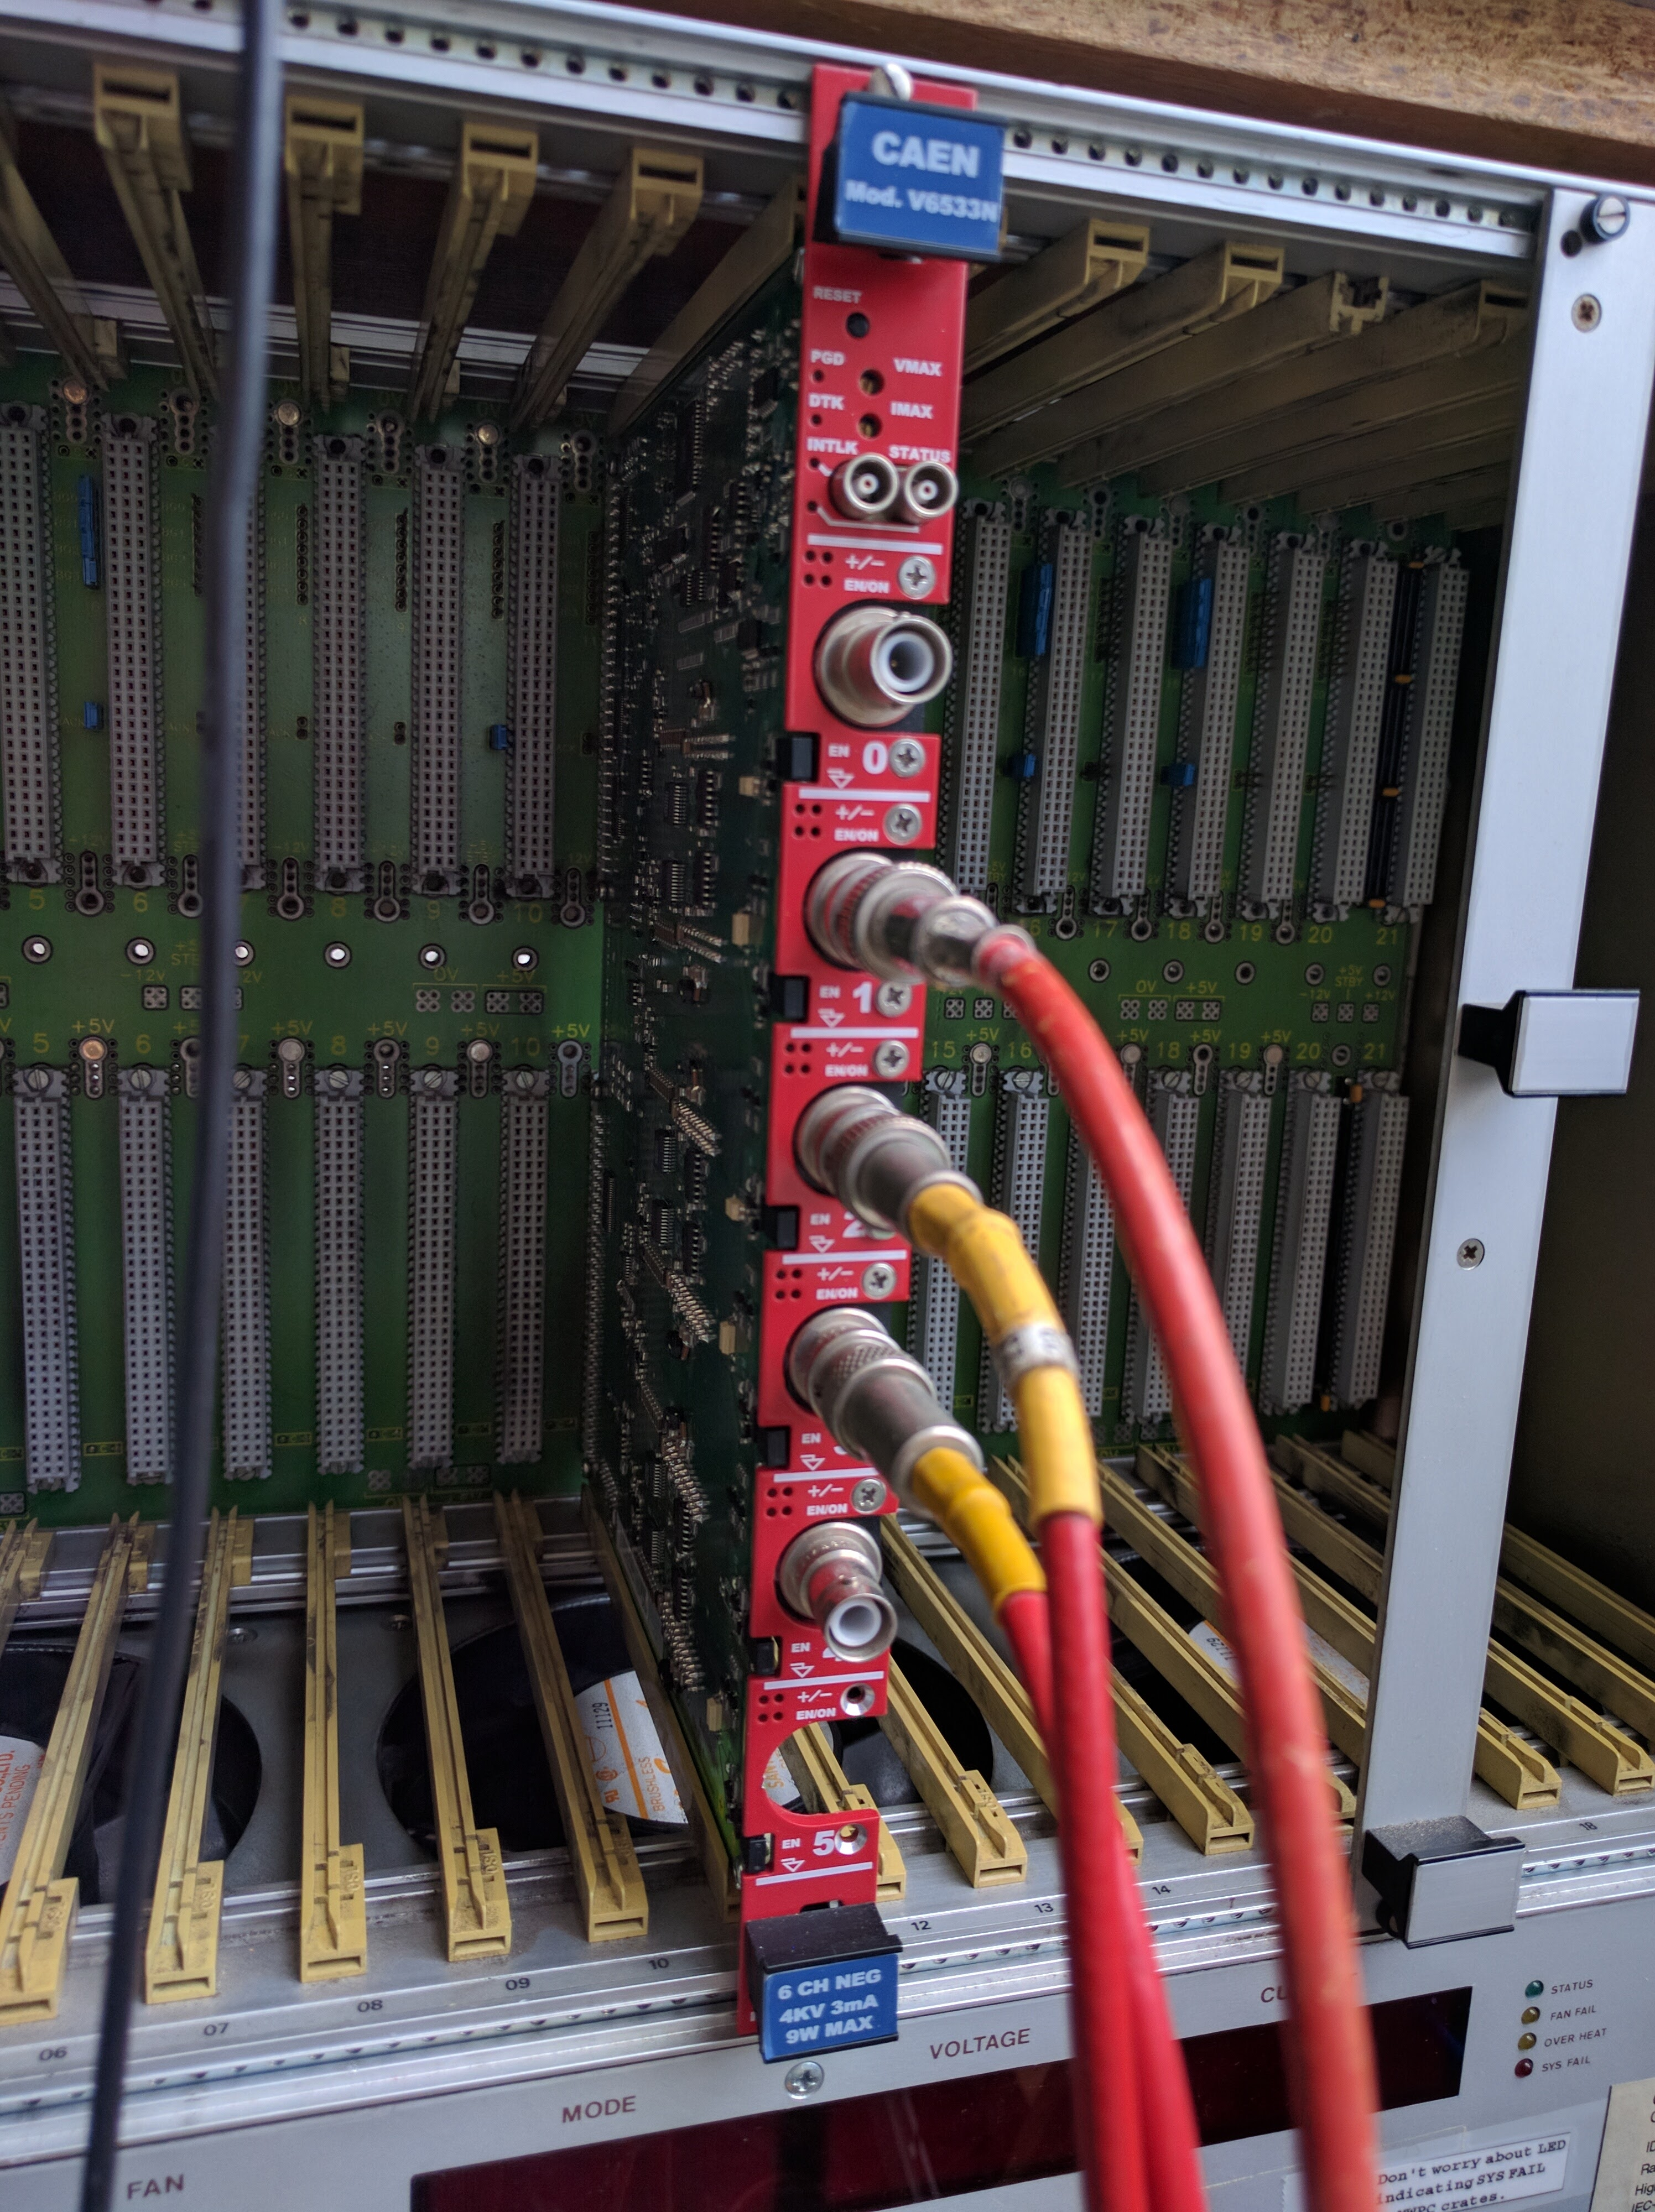
\includegraphics[width=0.39\textwidth]{img/III-1-arch/hv.jpg}
      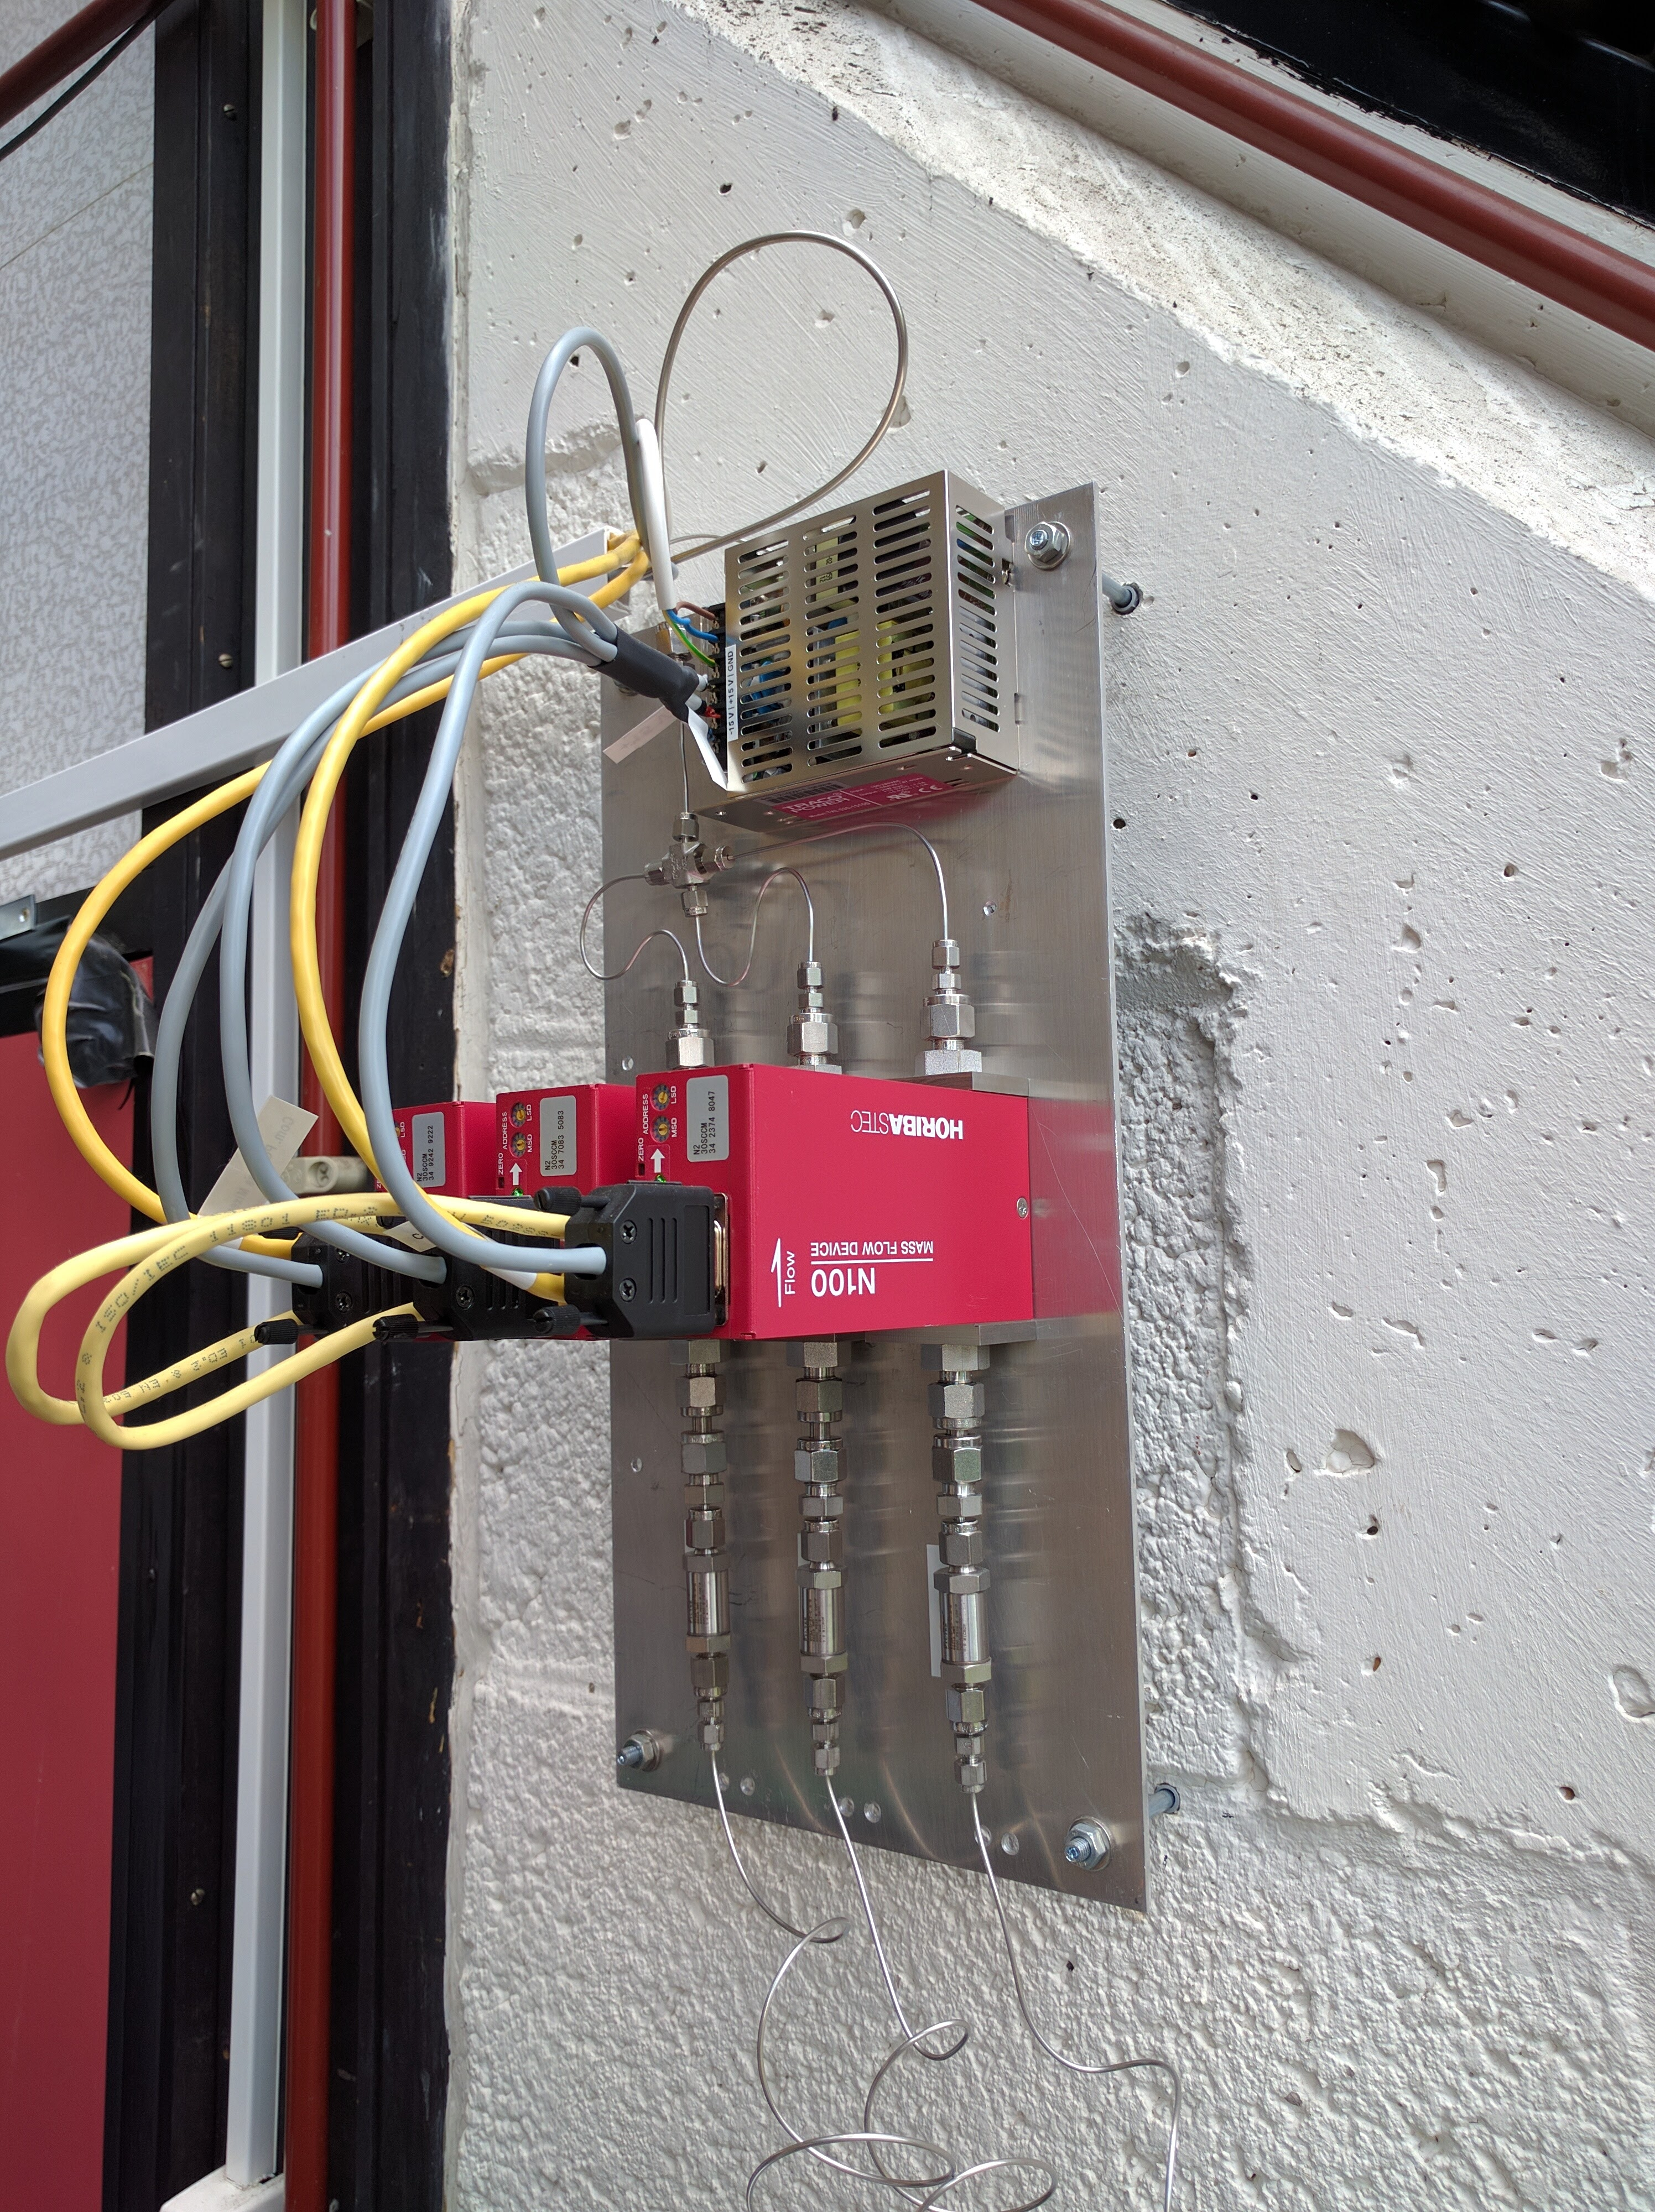
\includegraphics[width=0.39\textwidth]{img/III-1-arch/gas.jpg}
      \caption{}
      \label{fig:III-1-gas-hv}
    \end{figure}

  \section{The Infrastructure of the System}

    To control and monitor the GEM detectors, high voltage, and gas systems, a custom solution was developed around a web interface. The latter allows the user to change parameters of the runs, visualize the evolution of the settings, access logs, etc. All this information is stored in a database located on the central computing node which also hosts the web server. The database is the communication interface between all elements. It stores requests, responses, statuses, etc. From the database, a second computer located near the experimental setup extracts the parameters that need to be set on the high voltage and gas system and handles the communication protocol with these two components. This infrastructure remained unchanged while the data readout of the GEMs evolved with time.

    \subsection{The Web Interface}

      Controlling and monitoring the elements of the system is done through a web interface which makes heavy use of JavaScript. The web server runs on NodeJS, which allows JavaScript to be executed on the back-end, and communicates with the client through Socket.IO, an implementation of the WebSocket technology which provides real-time messaging. The rendering of the page is done using Bootstrap for the design and AngularJS for the data handling. Using these technologies, the web interface provides a responsive and user friendly application. \\

      The application is divided in three areas: the run control, high voltage monitoring, and gas monitoring. The run control is where parameters of the system are set when starting a new run. The system is constantly in run status even when the voltages are off or the gas disconnected. In order to differentiate data taking runs from stand-by runs, a logbook can be accessed to retrieve the parameters of the system. \\

      To monitor the parameters during a run, the user has to use home page to access a summary of the run, or the high voltage and gas pages for more details. These list the current status of the registers and monitoring valus which can be plotted. Figure \ref{fig:III-1-app} is a list of screenshots from the web application with the home page on the top left, run page on the top right, high voltage page on the bottom left, and gas page on the bottom right. Each page defines alarms that will modify the layout of the interface if error occurs, such as incorrect values stored in the system, over heating, etc. \\

      Every action taken or value read is respectively stored or read from the database. The web interface is the link between the user and the latter.

      \begin{figure}[h!]
        \centering
        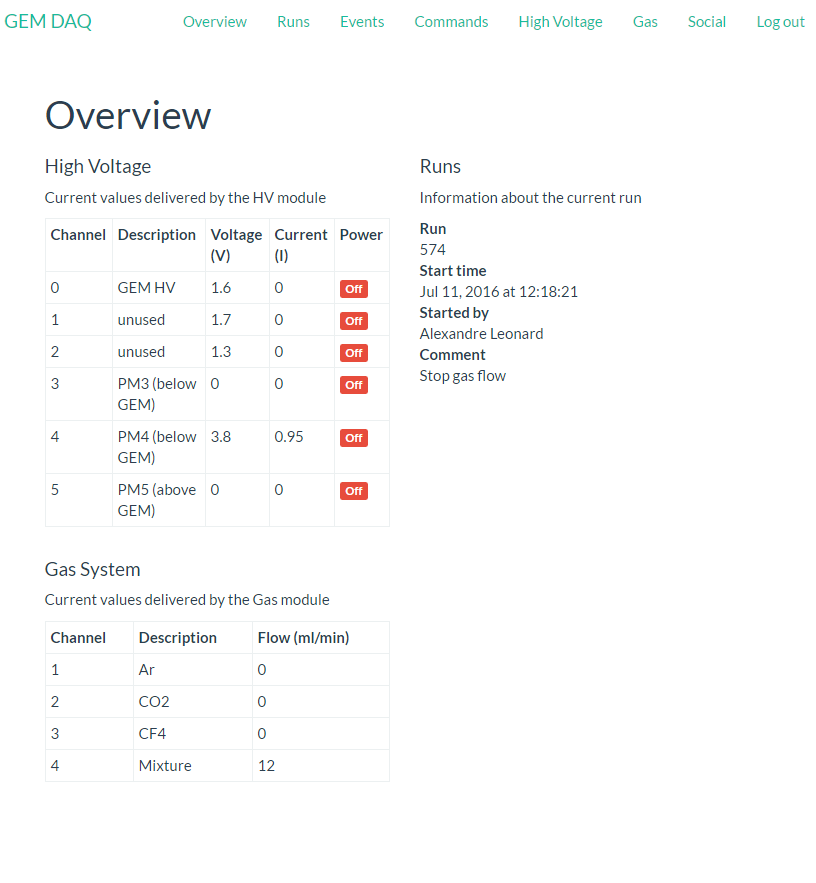
\includegraphics[width=0.49\textwidth]{img/III-1-arch/app-home.png}
        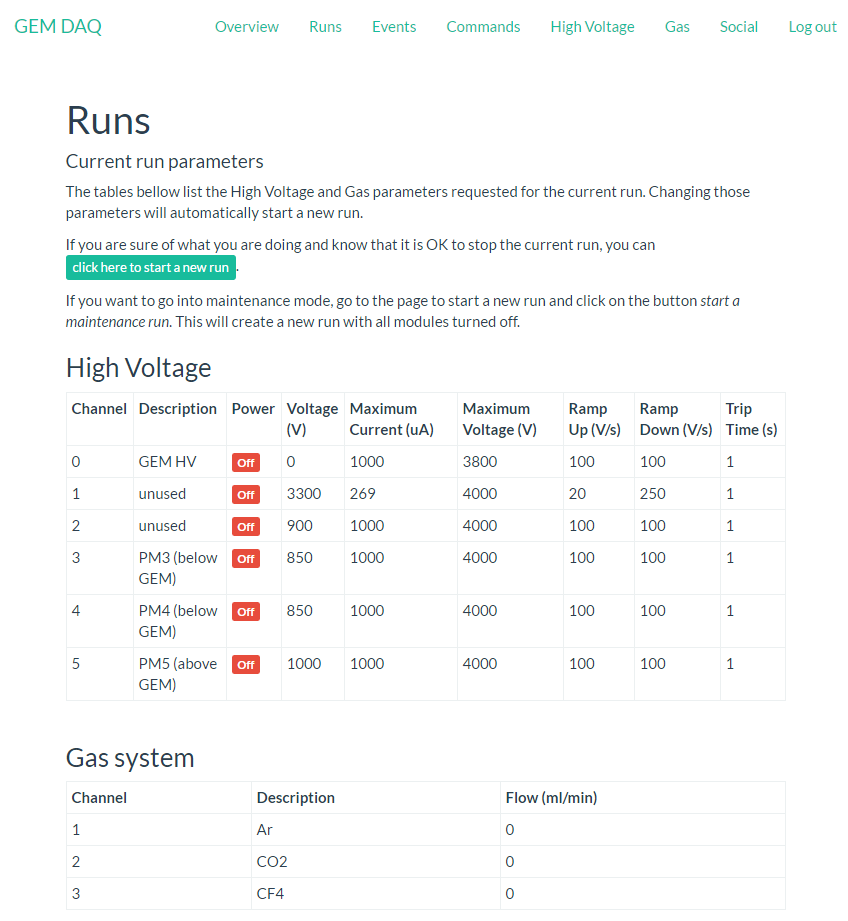
\includegraphics[width=0.49\textwidth]{img/III-1-arch/app-runs.png} \\
        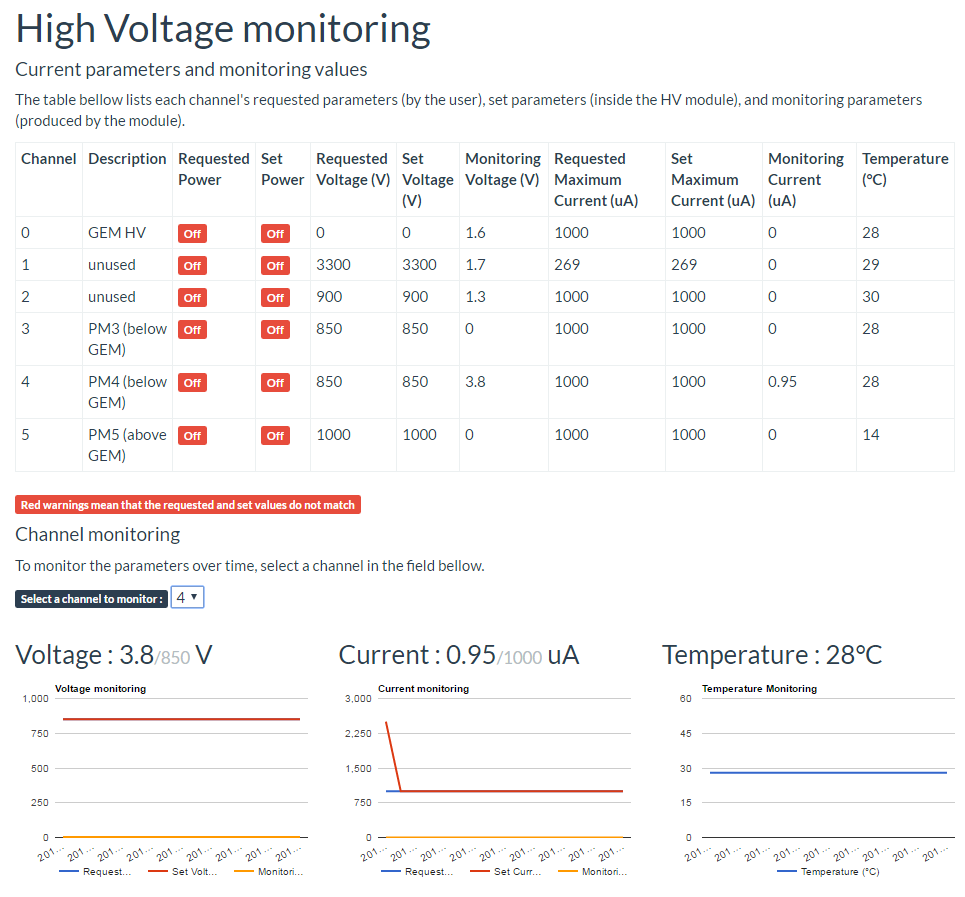
\includegraphics[width=0.49\textwidth]{img/III-1-arch/app-hv.png}
        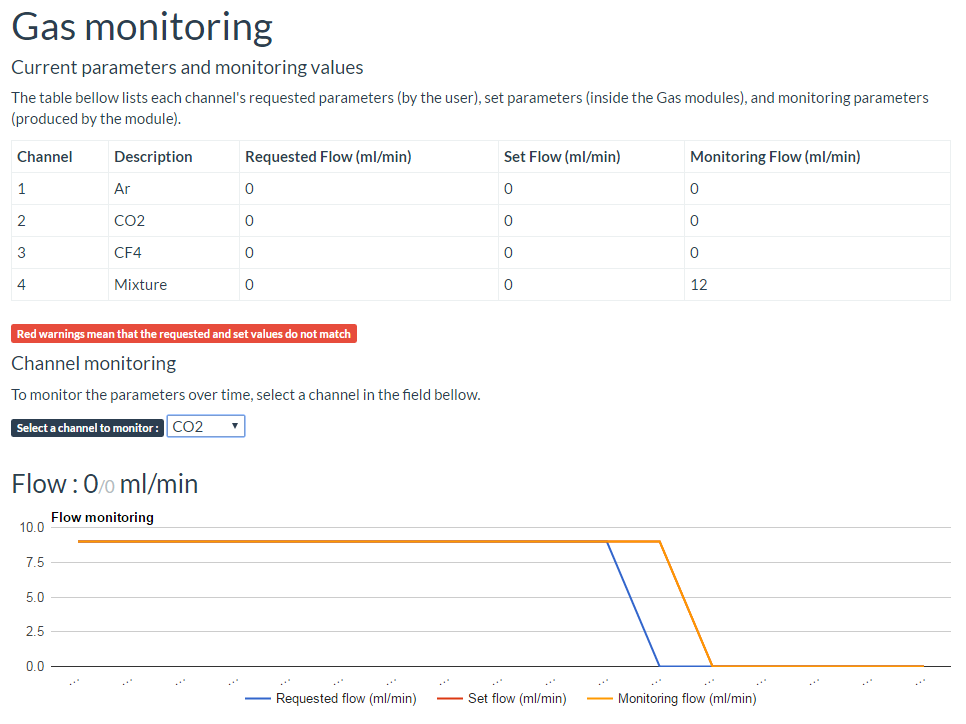
\includegraphics[width=0.49\textwidth]{img/III-1-arch/app-gas.png}
        \caption{}
        \label{fig:III-1-app}
      \end{figure}

    \subsection{The Central Computing Node}

      The central computing node is located in a server rack far from the experimental setup. It holds the web server and the MySQL database. its main role is to log every action and store the monitoring data. It is the bottleneck of the system which limits communication throughput as it has to operate various operations on the database for each request which are relatively slow.

    \subsection{The High Voltage and Gas Controller}

      The communication between the database and the high voltage and gas systems is done through a computer placed in a rack near the experimental setup. Custom software was developped by the ULB DAQ team to communicate with the VME crate and the mass flow controllers. CAEN provides an integrated library to perform read/write operations on the crate which is used to apply the parameters stored in the database. Communication with the flow meters is done through UART in the same application.

  \section{A First Prototype using the Xilinx SP601 Development Board}

    The first prototype of the DAQ system was developed using a Xilinx SP601 development board which is equipped with a Xilinx Spartan-6 FPGA (XC6SLX16-2CSG324) similar to the one used on the first version of the OptoHybrid, 1 Gb of DDR2 SDRAM, an Ethernet PHY, a USB-to-UART bridge, and a VITA 57.1 FMC-LPC extension header. The SP601 was linked to a VFAT2 Hybrid mounted on the Triple-GEM detector through a specially designed board which plugged onto the FMC connector. On the other side, the SP601 was connected to the computer present in the rack. Figure \label{fig:III-1-sys-1} provides a schematic overview of the system and its components.

    \begin{figure}[h!]
      \centering
      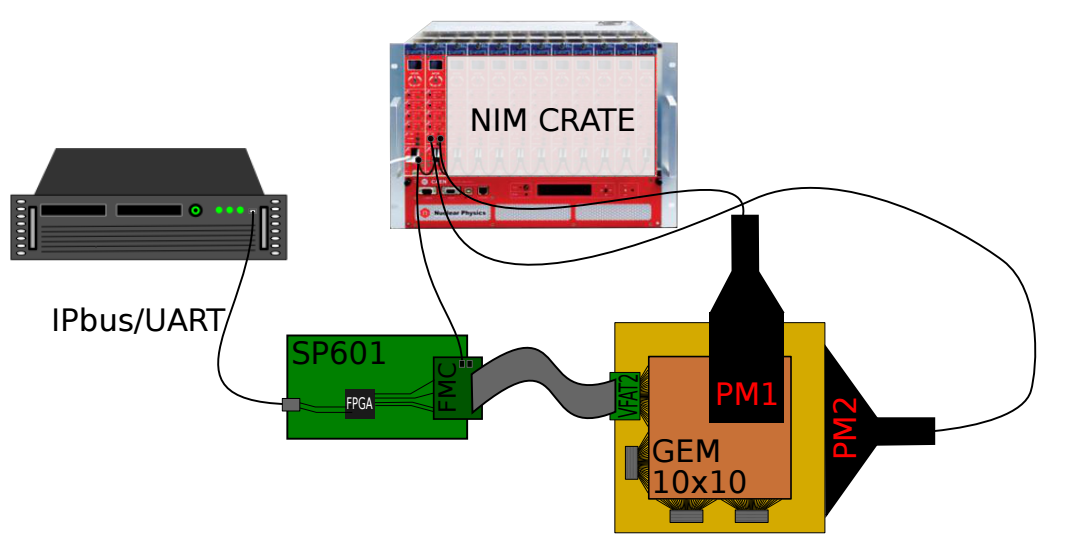
\includegraphics[width=0.8\textwidth]{img/III-1-arch/sys_1.png}
      \caption{SYS 1.}
      \label{fig:III-1-sys-1}
    \end{figure}

    \subsection{The VFAT2 FMC}

      The VFAT2 FMC is a small board which makes the connection between the SP601 and two VFAT2s, provides power to the boards, and is able to receive or send triggers through two LEMO connectors. It connects to the FMC header of the SP601 and forwards the signals of the VFAT2s to the FPGA.

      \begin{figure}[h!]
        \centering
        
\includegraphics[width=\textwidth]{img/empty.png}
        \caption{FMC.}
        \label{fig:III-1-fmc}
      \end{figure}

    \subsection{The Trigger and Tracking Paths}

      The trigger, defined as the coincidence of the top and bottom photomultipliers, is injected in the system through the LEMO connectors of the FMC board and redirected to the FPGA. It is then encrypted and forwarded to the VFAT2s as a T1 signal. The trigger data received from the VFAT2s is put on one bit using a logic-OR and transmitted over the second LEMO connector of the FMC board and used to measure timing delays. \\

      The tracking data of the VFAT2s is decoded and stored in a local buffer to be later read out by the MicroBlaze soft core processor implemented on the FPGA.

    \subsection{The MicroBlaze Soft Core Processor}

      MicroBlaze is an embedded 32-bit processor developed by Xilinx which can be implemented on the fabric of the FPGA. As it is not hard-coded in the silicon of the FPGA, it is said to be a soft core. Figure \ref{fig:III-1-microblaze} is a functional diagram of the architecture of the processor. The instruction buffer holds the instructions to be executed by the processor. They are decoded by the instruction decoder which forwards the operation the registers or to the various logic units: the Arithmetic Logic Unit (ALU) which performs integer operations, the Floating Point Unit (FPU) which performs floating point operations, etc. The result of the operation is either stored in the registers or forwarded on the data bus. Finally, new instructions are fetched on the instruction bus to be stored in the instruction buffer according to the program counter value which points to the next address to execute. The data and instruction buses use a 32-bit addressing scheme to retrieve data from the elements they are connected to and communicate with the components that attach to the processor. \\

      \begin{figure}[h!]
        \centering
        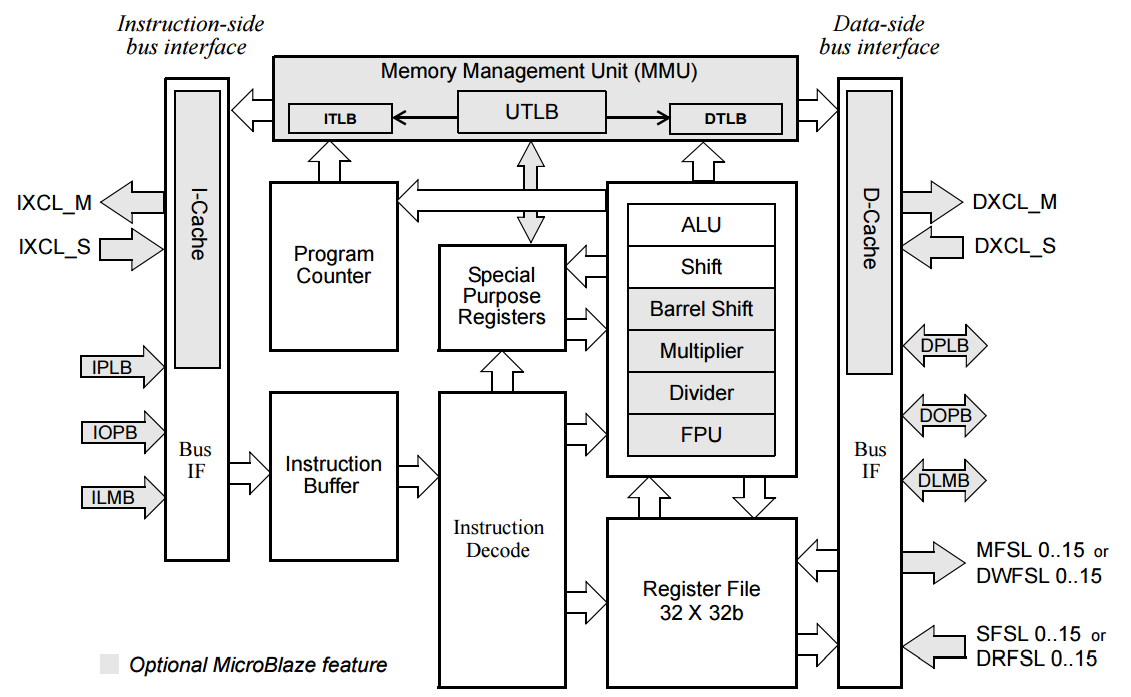
\includegraphics[width=\textwidth]{img/III-1-arch/microblaze.png}
        \caption{microblaze.}
        \label{fig:III-1-microblaze}
      \end{figure}

      To extend the computing power offered by the MicroBlaze processor, the data bus and instruction bus can be connected to other entities that are also implemented on the fabric of the FPGA. For example, a given address range of the instruction bus can be mapped to a memory controller which will interface with the onboard SDRAM to store the instructions of the program to run. The data bus on the other hand can be connected to Ethernet controllers, UART modules, etc to extended the IO capability of the processor. The way the instruction and data bus are mapped generated an address map file which describes the components attached to the processor. \\

      To control the processor and its components, a toolkit is provided by Xilinx to compile C or C++ code for the MicroBlaze. Each module also comes with a driver which is used in conjunction with the address map file to access the dedicated functions. Additional modules can be developed and connected to the MicroBlaze interface, which has been done to control the buffer holding the tracking data of the VFAT2s. The module is composed of VHDL code to control the buffer on the fabric of the FPGA and of a driver written in C to provide high-level functions to access the data. \\

      The final design of the MicroBlaze processor is composed of an external memory controller to store the program, an I2C controller to communicate with the slow control of the VFAT2, a dedicated module created to read out the tracking data, and a UART module to communicate with the computer located near the experimental setup.

    \subsection{IPBus over UART}

      The connection between the computer and the SP601 is done through UART over USB. The conversion between protocols is done through either drivers on the computer or a dedicated chip on the development board. The output of the chip is further connected to the MicroBlaze which receives interrupts whenever data is transmitted. \\

      UART is a full-duplex two-wires protocol: RX which receives data and TX which transmits data. The communicating parties are set on equal ground (no master or slave) and do not exchange a clock which means they have to agree on a sampling frequency before hand. The latter is the limiting factor as uncorrelated clocks will have slightly different frequencies and thus induce errors when sampling at high speeds. Therefore, UART is limited to speeds of 1 kHz which means data is transmitted at 100 bits per second. When the lines are idle, they are pulled up in order to indicate the presence of the other party. To initiate a communication, a start bit corresponding to a logic '0' is sent. Then follows the 8 bits of data with the LSB sent first. Finally, a stop bit equal to a logic '1' is sent, ensuring that during each communication a transition from '0' to '1' ensues. Figure \ref{fig:III-1-uart} shows the communication protocol with the relevant bit order. \\

      \begin{figure}[h!]
        \centering
        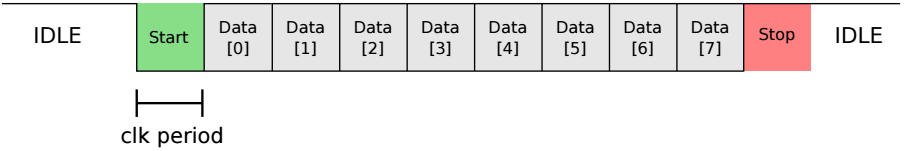
\includegraphics[width=0.8\textwidth]{img/III-1-arch/uart.png}
        \caption{uart.}
        \label{fig:III-1-uart}
      \end{figure}

      To control the systems, it was chosen to use an implementation of IPBus over UART to be as close as possible to later developments. To this end, dedicated software has been design for both the computer and the MicroBlaze. The software is flexible enough to either user a UART or an Ethernet interface, abstracting the transportation layer from the data. In the case of the UART implementation that was used, the 32-bit structure of the IPBus frame is decomposed in 8-bit packets. Each instruction is then recomposed by the MicroBlaze and forwarded to the corresponding module. The response is then sent back to the computer. \\

      The software in charge of the communication with the SP601 that is running on the computer is constantly polling the database for new requests to transmit. It also pulls data out of the tracking data buffers that it stores in the same database. The user can then visualize the events from the web interface or issue commands. Figure \ref{fig:III-1-app-cmd} is a screenshot of the interface that allows the user to send commands and read the response from the system.

      \begin{figure}[h!]
        \centering
        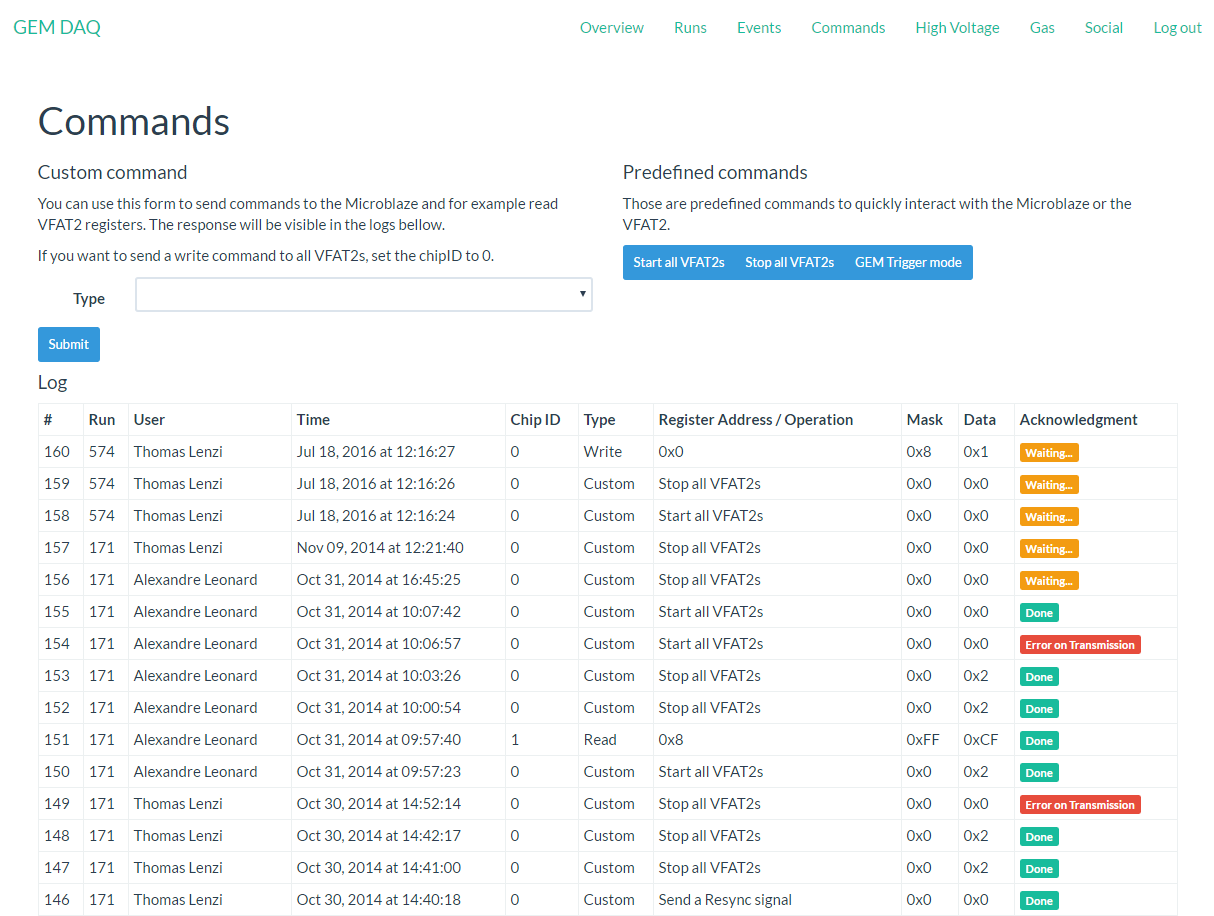
\includegraphics[width=0.7\textwidth]{img/III-1-arch/app-cmd.png}
        \caption{App cmd.}
        \label{fig:III-1-app-cmd}
      \end{figure}

  \section{Upgrade of the System using the GLIB}

    When the GLIB became available, developments focused on the backend electronics and software moved from an IPBus UART to an IPBus Ethernet implementation. As the GLIB is also equipped with an FMC connector, it was decided to use it as frontend module coupled with the VFAT2 FMC already used in the first prototype. The choice to separate the system instead of implementing the full design on one GLIB was made to develop knowledge with respect to the use of optical links. Figure \ref{fig:III-1-sys-2} displays the configuration of the system using two GLIBs as readout boards. \\

    \begin{figure}[h!]
      \centering
      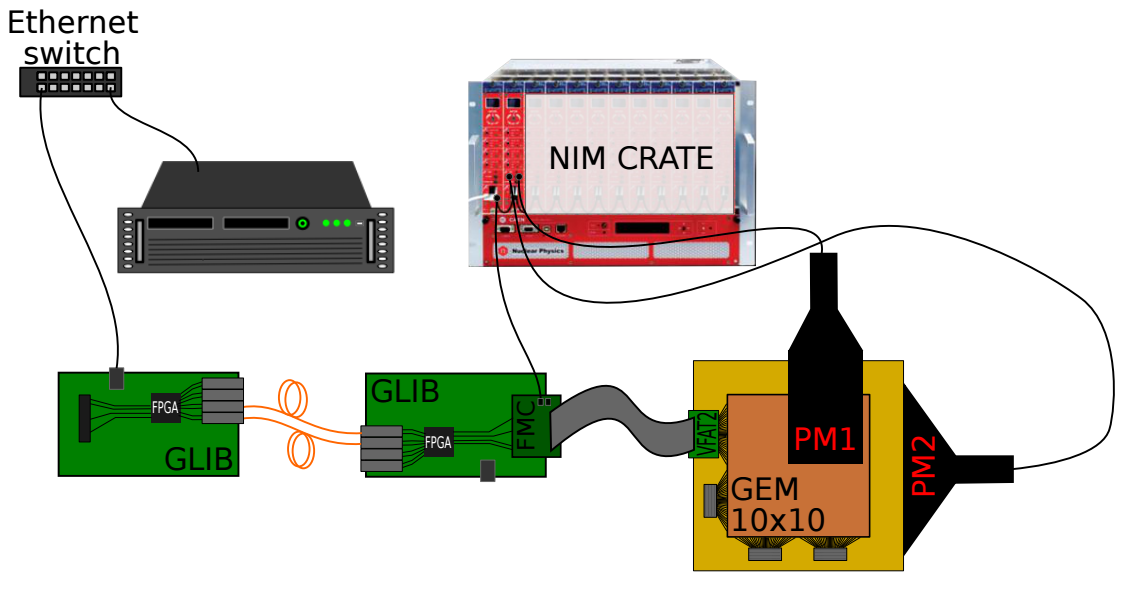
\includegraphics[width=0.8\textwidth]{img/III-1-arch/sys_2.png}
      \caption{SYS 2.}
      \label{fig:III-1-sys-2}
    \end{figure}

    

  \section{Final System using the First Prototype of the OptoHybrid}

    \begin{figure}[h!]
      \centering
      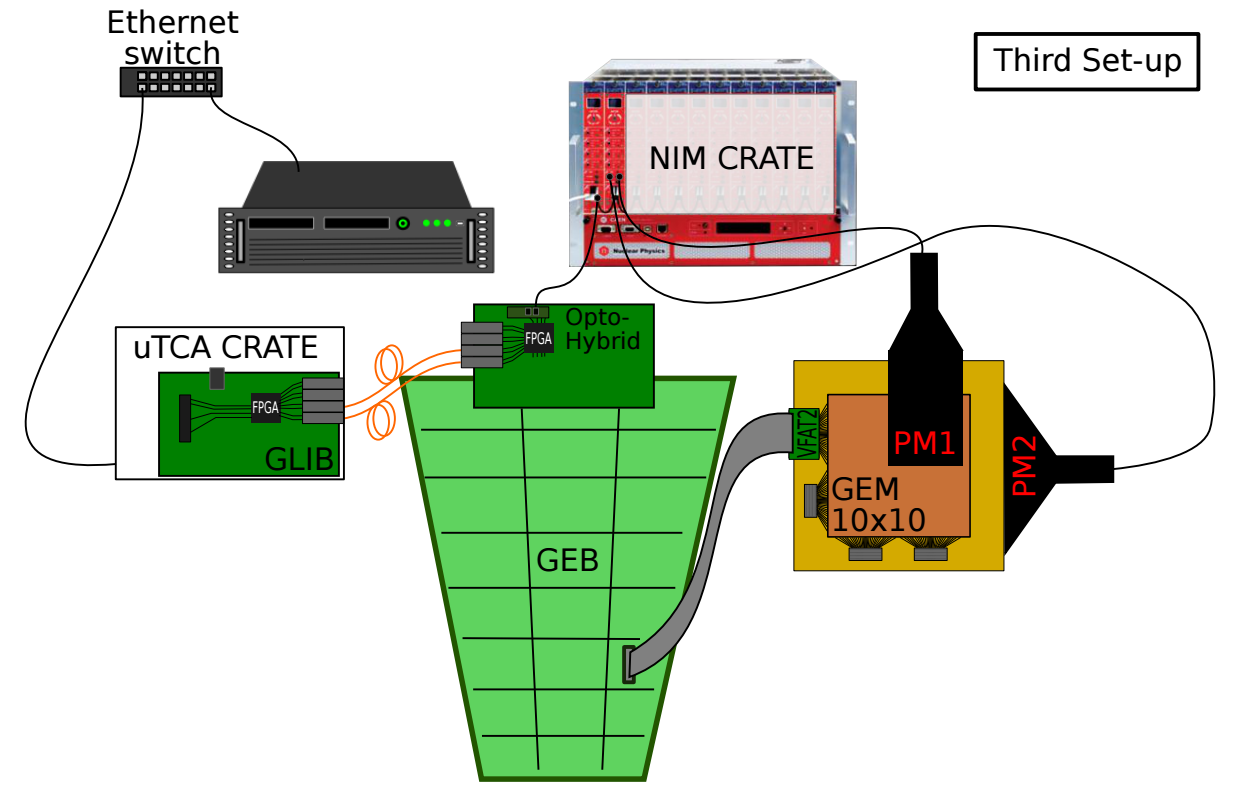
\includegraphics[width=0.8\textwidth]{img/III-1-arch/sys_3.png}
      \caption{SYS 3.}
      \label{fig:III-1-sys-3}
    \end{figure}























  \section{Conclusion}
